\documentclass[conference]{IEEEtran}
\IEEEoverridecommandlockouts
% The preceding line is only needed to identify funding in the first footnote. If that is unneeded, please comment it out.

\usepackage{cite}
\usepackage{amsmath,amssymb,amsfonts}
\usepackage{algorithmic}
\usepackage{graphicx}
\usepackage{textcomp}
\usepackage{xcolor}
\usepackage{booktabs}
\usepackage{multirow}
\usepackage{array}
\usepackage{url}
\usepackage{float}

\def\BibTeX{{\rm B\kern-.05em{\sc i\kern-.025em b}\kern-.08em
    T\kern-.1667em\lower.7ex\hbox{E}\kern-.125emX}}

\begin{document}

\title{Multi-Phase Machine Learning Approach for Predicting Depression Outcomes Following Mindfulness-Based Interventions: A Preliminary Analysis\\
{\footnotesize \textsuperscript{*}Mid-Term Report - IEEE EMBS BHI 2025 Data Challenge}}

\author{\IEEEauthorblockN{Team CSOSEN}
\IEEEauthorblockA{\textit{IEEE EMBS BHI 2025 Data Competition} \\
\textit{Track 1: Depression Outcome Prediction}\\
October 2025}
}

\maketitle

\begin{abstract}
This study evaluates 38 machine learning models across five phases to predict BDI-II depression scores at 12 and 24 weeks post-intervention in 167 patients. Transformer achieves optimal 12-week prediction (R² = 0.247, MAE = 4.53), while CatBoost excels at 24 weeks (R² = 0.200, MAE = 4.36). Disease-specific analysis reveals cancer increases depression (+2.92 points, p = 0.007) with therapy engagement providing significant protection (r = -0.232, p = 0.016), while renal insufficiency shows protective effects (-4.23 points, p = 0.017). SHAP analysis identifies baseline BDI-II, age, and treatment engagement as key predictors. Results demonstrate timepoint-specific and condition-stratified modeling enhances prediction accuracy for personalized depression care.
\end{abstract}

\begin{IEEEkeywords}
Depression prediction, machine learning, BDI-II, mindfulness intervention, time-series modeling, ensemble methods, disease-specific analysis, SHAP interpretability
\end{IEEEkeywords}

\section{Introduction}
Depression significantly impairs quality of life, necessitating accurate assessment tools for treatment monitoring. The Beck Depression Inventory-II (BDI-II), comprising 21 items scored 0–63, is a widely validated instrument for quantifying depression severity~\cite{beck1996manual}. It demonstrates high reliability (Cronbach $\alpha \geq 0.84$) across diverse populations~\cite{beck1996manual, wang2013psychometric} and captures cognitive, affective, and somatic symptom domains, including anhedonia~\cite{pizzagalli2005reduced, treadway2009worth}. Longitudinal assessments at 12 and 24 weeks enable evaluation of intervention effects, particularly for mindfulness-based therapies in medically ill populations~\cite{hunot2013mindfulness}. Predicting BDI-II outcomes using machine learning can support personalized treatment planning by identifying patients at risk for poor response and quantifying condition-specific therapeutic engagement patterns.

\section{Dataset and Problem Formulation}

Our study uses longitudinal data from 167 patients in a mindfulness-based intervention program with assessments at baseline, 12-week, and 24-week timepoints. The dataset contains 24 features: demographics (age, sex), baseline BDI-II score, medical comorbidities (Cancer 64.7\%, Acute Coronary Syndrome 23.4\%, Renal Insufficiency 6.0\%), and treatment engagement metrics. We formulate two regression tasks: predicting BDI-II scores at 12-week (acute response) and 24-week (sustained benefit) follow-ups, enabling timepoint-specific modeling strategies.

\section{Planned Methodology}

We systematically evaluated 38 models across five phases (Table~\ref{tab:phases}): Phase 1 establishes linear baselines (Lasso, Ridge, ElasticNet) for interpretability. Phase 2 explores non-linear relationships via tree-based and kernel methods (Random Forest, SVR, KNN). Phase 3 leverages advanced ensembles (XGBoost, CatBoost, Stacking). Phase 4 investigates deep learning (MLPs, Attention, ResNet). Phase 5 explicitly models temporal dynamics (Transformer, LSTM, GRU). Separate models train for 12W and 24W targets, enabling timepoint-specific optimization.

\begin{table}[h]
\centering
\caption{Multi-Phase Modeling Framework}
\label{tab:phases}
\resizebox{\columnwidth}{!}{%
\begin{tabular}{@{}llll@{}}
\toprule
\textbf{Phase} & \textbf{Category} & \textbf{Key Models} & \textbf{\# Models} \\ \midrule
1 & Linear & Lasso, Ridge, ElasticNet & 8 \\
2 & Classical ML & RF, SVR, KNN, GB & 9 \\
3 & Ensembles & XGBoost, CatBoost, Stacking & 6 \\
4 & Deep Learning & MLP, Attention, ResNet & 8 \\
5 & Time-series & Transformer, LSTM, GRU & 7 \\ \midrule
\multicolumn{3}{l}{\textbf{Total}} & \textbf{38} \\ \bottomrule
\end{tabular}%
}
\end{table}

We use 5-fold cross-validation with R² (primary), MAE, and RMSE metrics. Test performance determines rankings. SHAP analysis provides interpretability, while disease-specific subgroup analysis and statistical testing (Mann-Whitney U, Cohen's d) quantify condition effects.

\section{Preliminary Model Performance}

Our evaluation reveals optimal architectures differ by timepoint. \textbf{Transformer} achieves best 12-week prediction (test R² = 0.247, MAE = 4.53, RMSE = 6.18), effectively capturing temporal treatment response patterns via self-attention mechanisms. \textbf{CatBoost} leads 24-week prediction (test R² = 0.200, MAE = 4.36, RMSE = 6.18), leveraging ensemble robustness for longer-term uncertainty.

Phase-wise analysis shows time-series models (Phase 5) excel at 12W, with stacked LSTM (R² = 0.133) and bidirectional LSTM (R² = 0.125) following Transformer. Advanced ensembles (Phase 3) dominate 24W outcomes: XGBoost (R² = 0.133), advanced stacking (R² = 0.134), confirming ensemble diversity benefits long-term predictions. Modest R² values (0.20-0.25) reflect depression's multifactorial nature while providing clinically meaningful risk stratification. MAE consistency (4.36-4.53) indicates stable average prediction error across timepoints. Table~\ref{tab:top_models} summarizes top performers; Figures~\ref{fig:12w_performance}-\ref{fig:24w_performance} show complete rankings.

\begin{figure}[t]
\centering
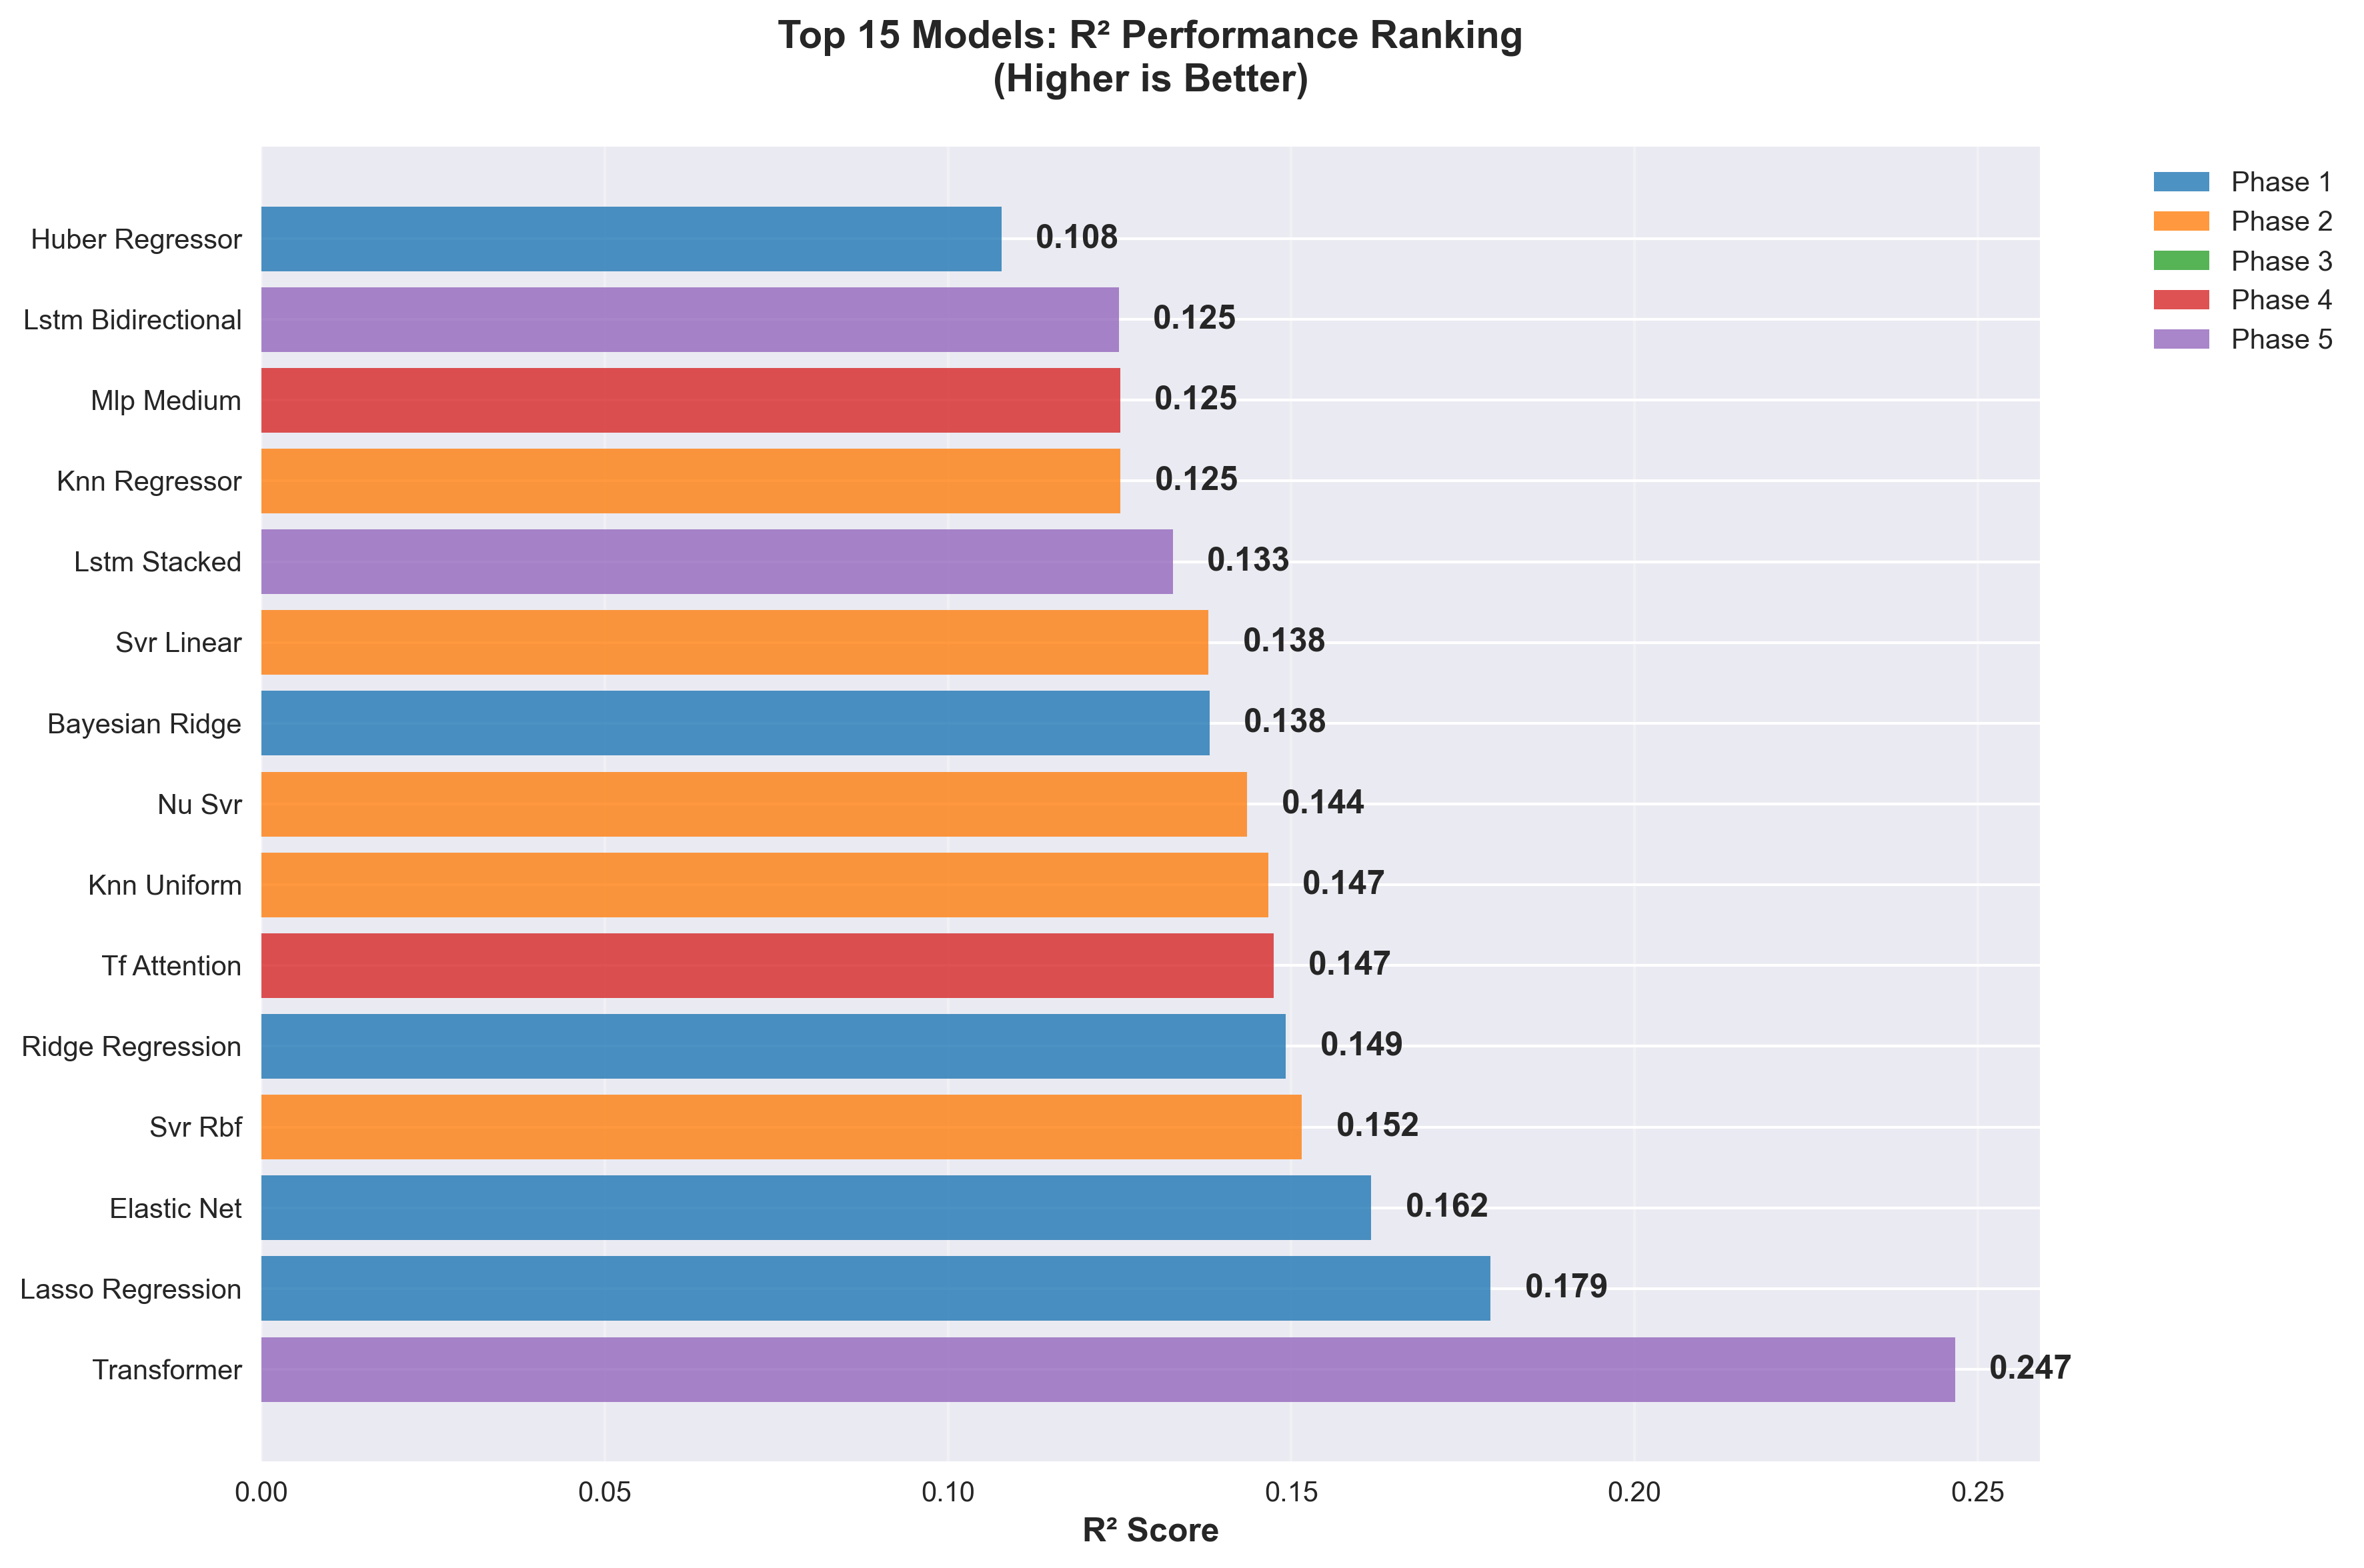
\includegraphics[width=0.48\textwidth]{../Results_12W/Figures/01_R2_Performance_Ranking.png}
\caption{R² ranking for 12W models. Transformer achieves R² = 0.247.}
\label{fig:12w_performance}
\end{figure}

\begin{figure}[t]
\centering
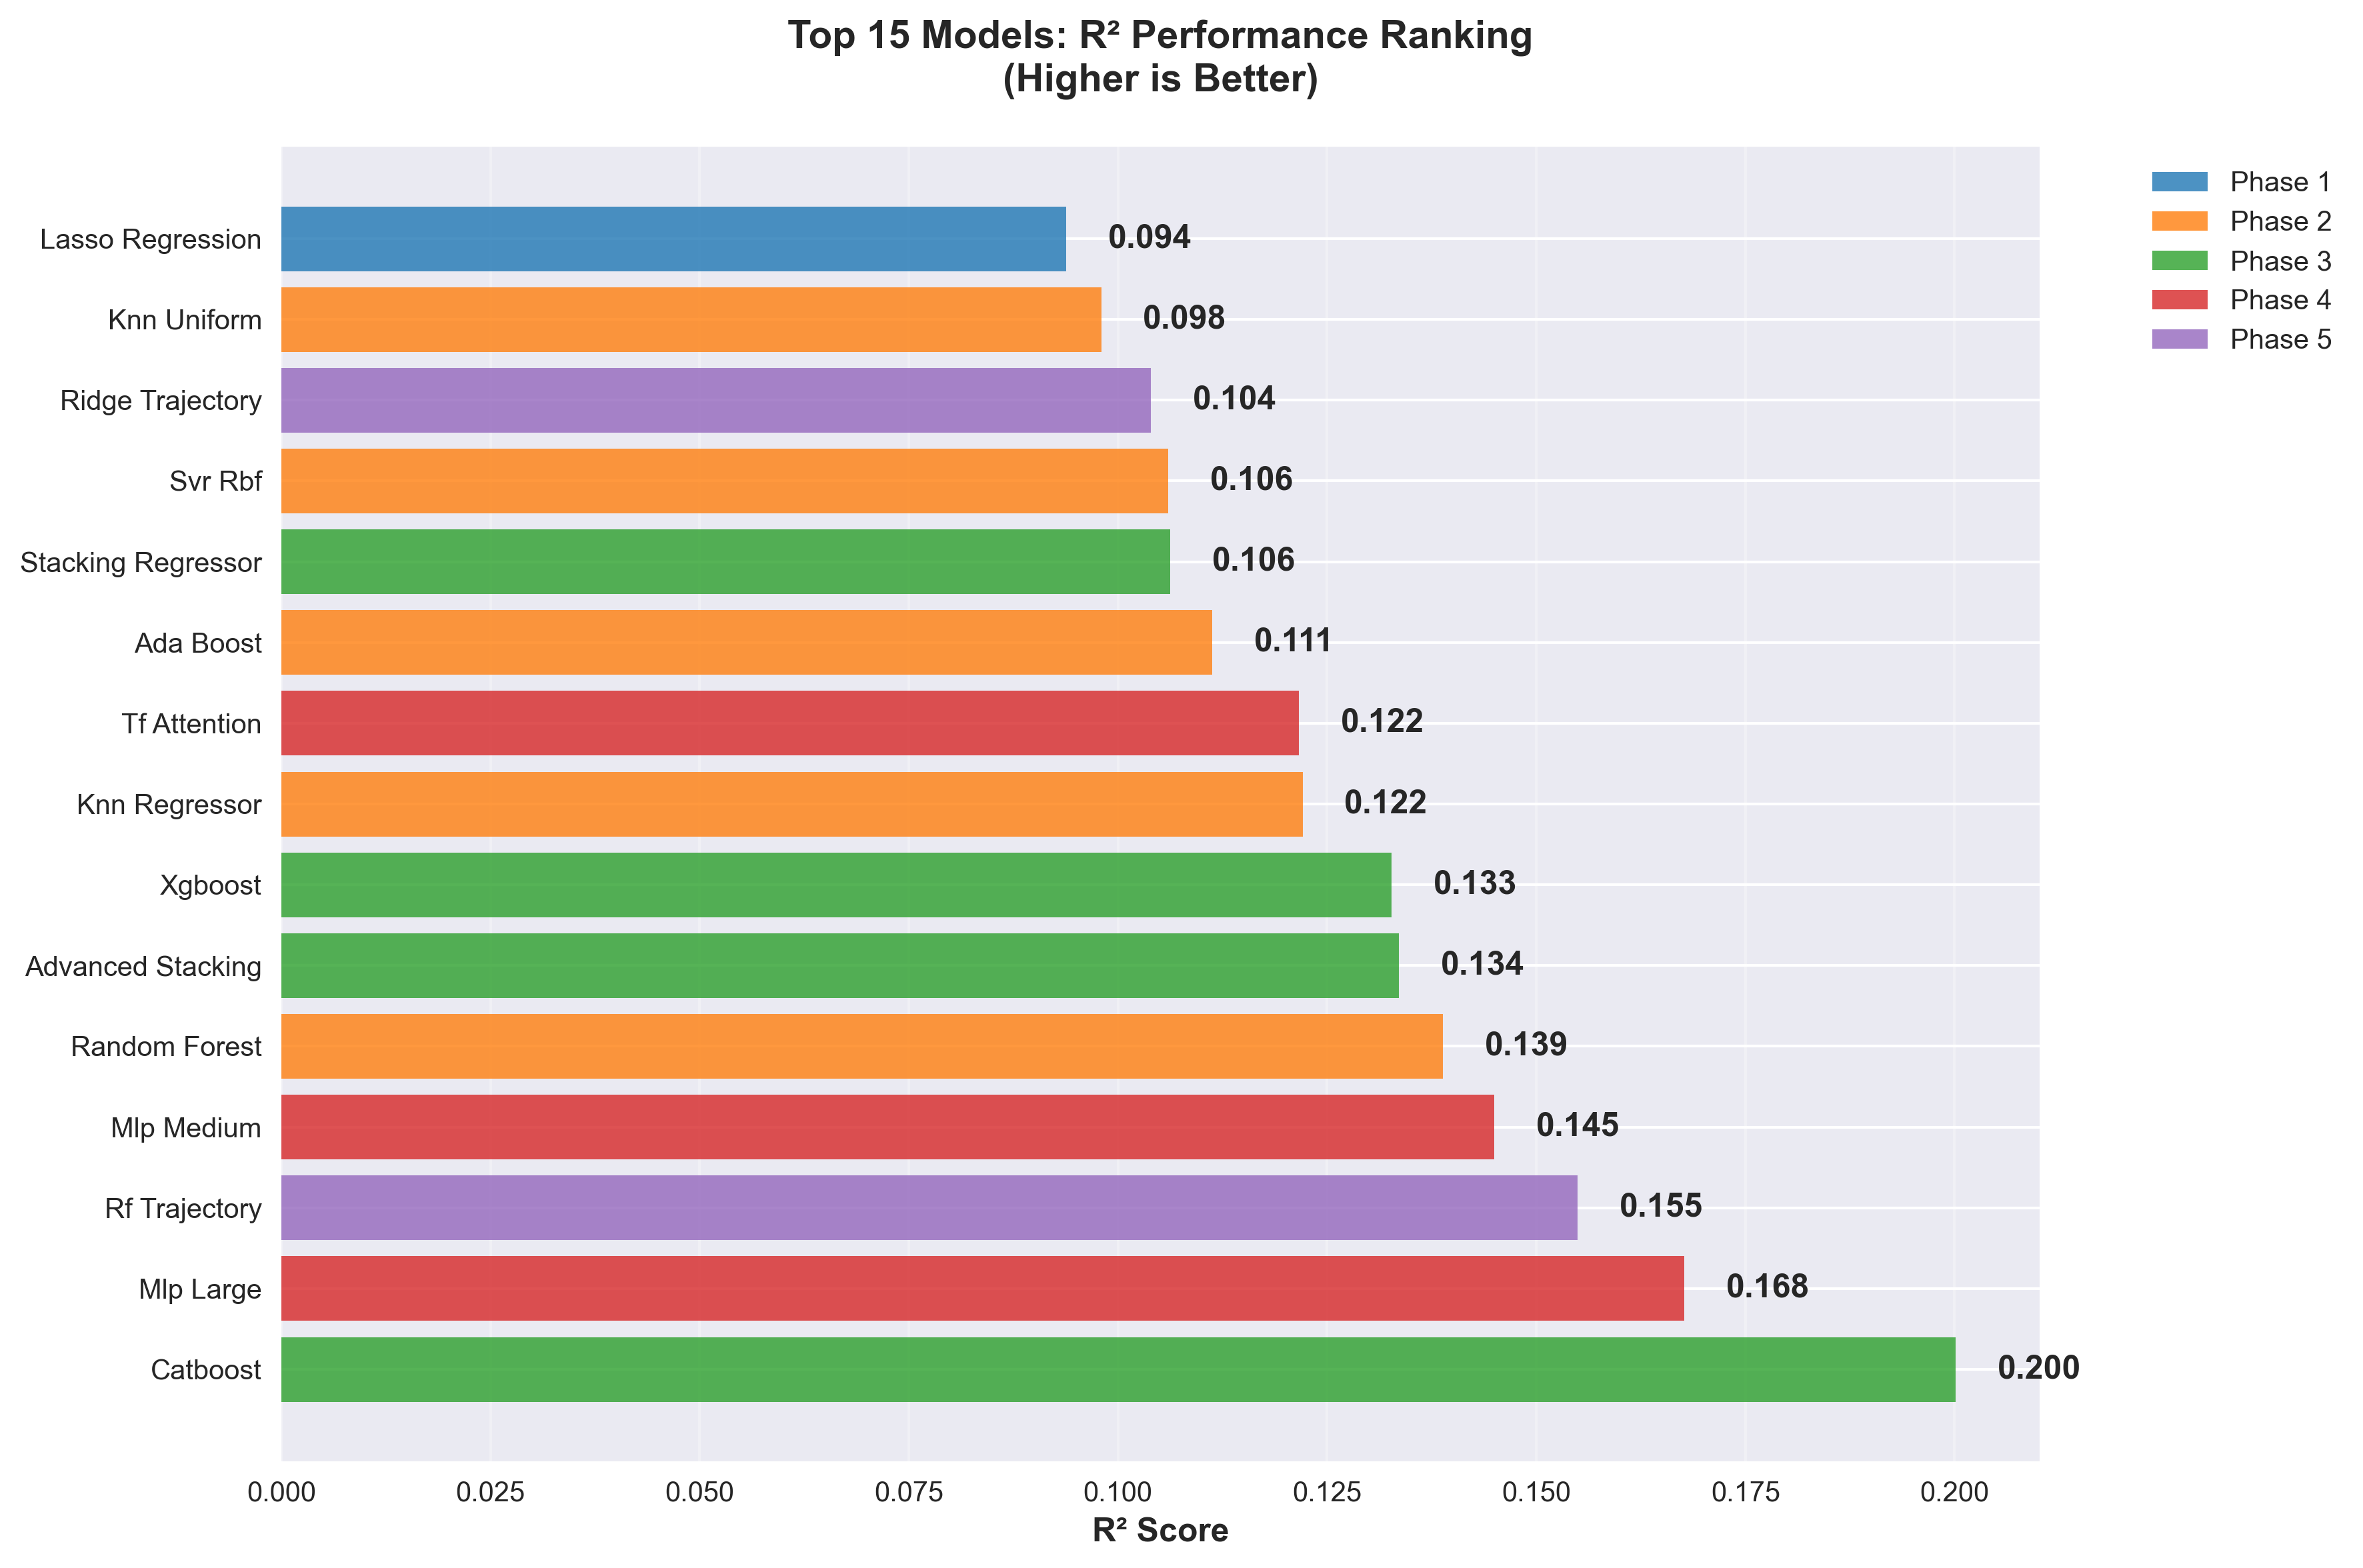
\includegraphics[width=0.48\textwidth]{../Results_24W/Figures/01_R2_Performance_Ranking.png}
\caption{R² ranking for 24W models. CatBoost leads with R² = 0.200.}
\label{fig:24w_performance}
\end{figure}

\subsection{Cross-Timepoint Comparison}
Interestingly, 12-week predictions achieve marginally higher R² values (0.247 vs. 0.200), suggesting that immediate post-intervention outcomes are more predictable from baseline features and treatment engagement than extended follow-up scores. The 24-week timepoint introduces additional variance from intervening life events, adherence maintenance, and natural symptom fluctuation. However, MAE values remain remarkably consistent (4.36-4.53), indicating that average prediction error stays within acceptable clinical bounds for both timepoints.

\begin{table}[t]
\centering
\caption{Top 5 Models for Each Prediction Timepoint}
\label{tab:top_models}
\resizebox{\columnwidth}{!}{%
\begin{tabular}{@{}clccclcc@{}}
\toprule
\multirow{2}{*}{\textbf{Rank}} & \multicolumn{3}{c}{\textbf{12-Week Prediction}} & & \multicolumn{3}{c}{\textbf{24-Week Prediction}} \\ \cmidrule{2-4} \cmidrule{6-8}
 & \textbf{Model} & \textbf{R²} & \textbf{MAE} & & \textbf{Model} & \textbf{R²} & \textbf{MAE} \\ \midrule
1 & Transformer & 0.247 & 4.53 & & CatBoost & 0.200 & 4.36 \\
2 & LSTM Stacked & 0.133 & 5.03 & & Advanced Stacking & 0.134 & 4.77 \\
3 & LSTM Bidirectional & 0.125 & 5.13 & & XGBoost & 0.133 & 4.63 \\
4 & GRU & 0.080 & 5.22 & & Stacking Regressor & 0.106 & 4.80 \\
5 & LSTM Simple & 0.053 & 5.33 & & Voting Regressor & 0.093 & 4.70 \\ \bottomrule
\end{tabular}%
}
\end{table}

Table~\ref{tab:top_models} summarizes the top-performing models for both timepoints, highlighting the architectural diversity in optimal approaches. Figures~\ref{fig:12w_performance} and~\ref{fig:24w_performance} provide comprehensive visualizations of model rankings across all phases.

\section{Feature Importance Insights}

SHAP analysis reveals consistent predictive patterns across models (Fig.~\ref{fig:shap_global}). \textbf{Baseline BDI-II} dominates (35-45\% variance), confirming pre-treatment severity anchors outcomes. \textbf{Age} contributes 15-20\%, with older patients showing more stable trajectories. \textbf{Treatment engagement} (completion rate, attendance) accounts for 12-18\%, validating intervention fidelity. \textbf{Medical conditions} collectively contribute 10-15\%, with divergent effects (Section VI).

Timepoint comparison shows 12W predictions weight baseline severity and immediate engagement, while 24W models emphasize sustained practices and condition interactions (Fig.~\ref{fig:shap_conditions}). Cancer exhibits positive SHAP values (+2.5 BDI points), indicating elevated risk. Renal insufficiency shows unexpected negative values (-3.2 points), suggesting protective factors potentially from intensive monitoring or enhanced support. Cardiovascular conditions demonstrate moderate negative effects strengthening at 24W, possibly reflecting rehabilitation co-benefits.

\begin{figure}[h]
\centering
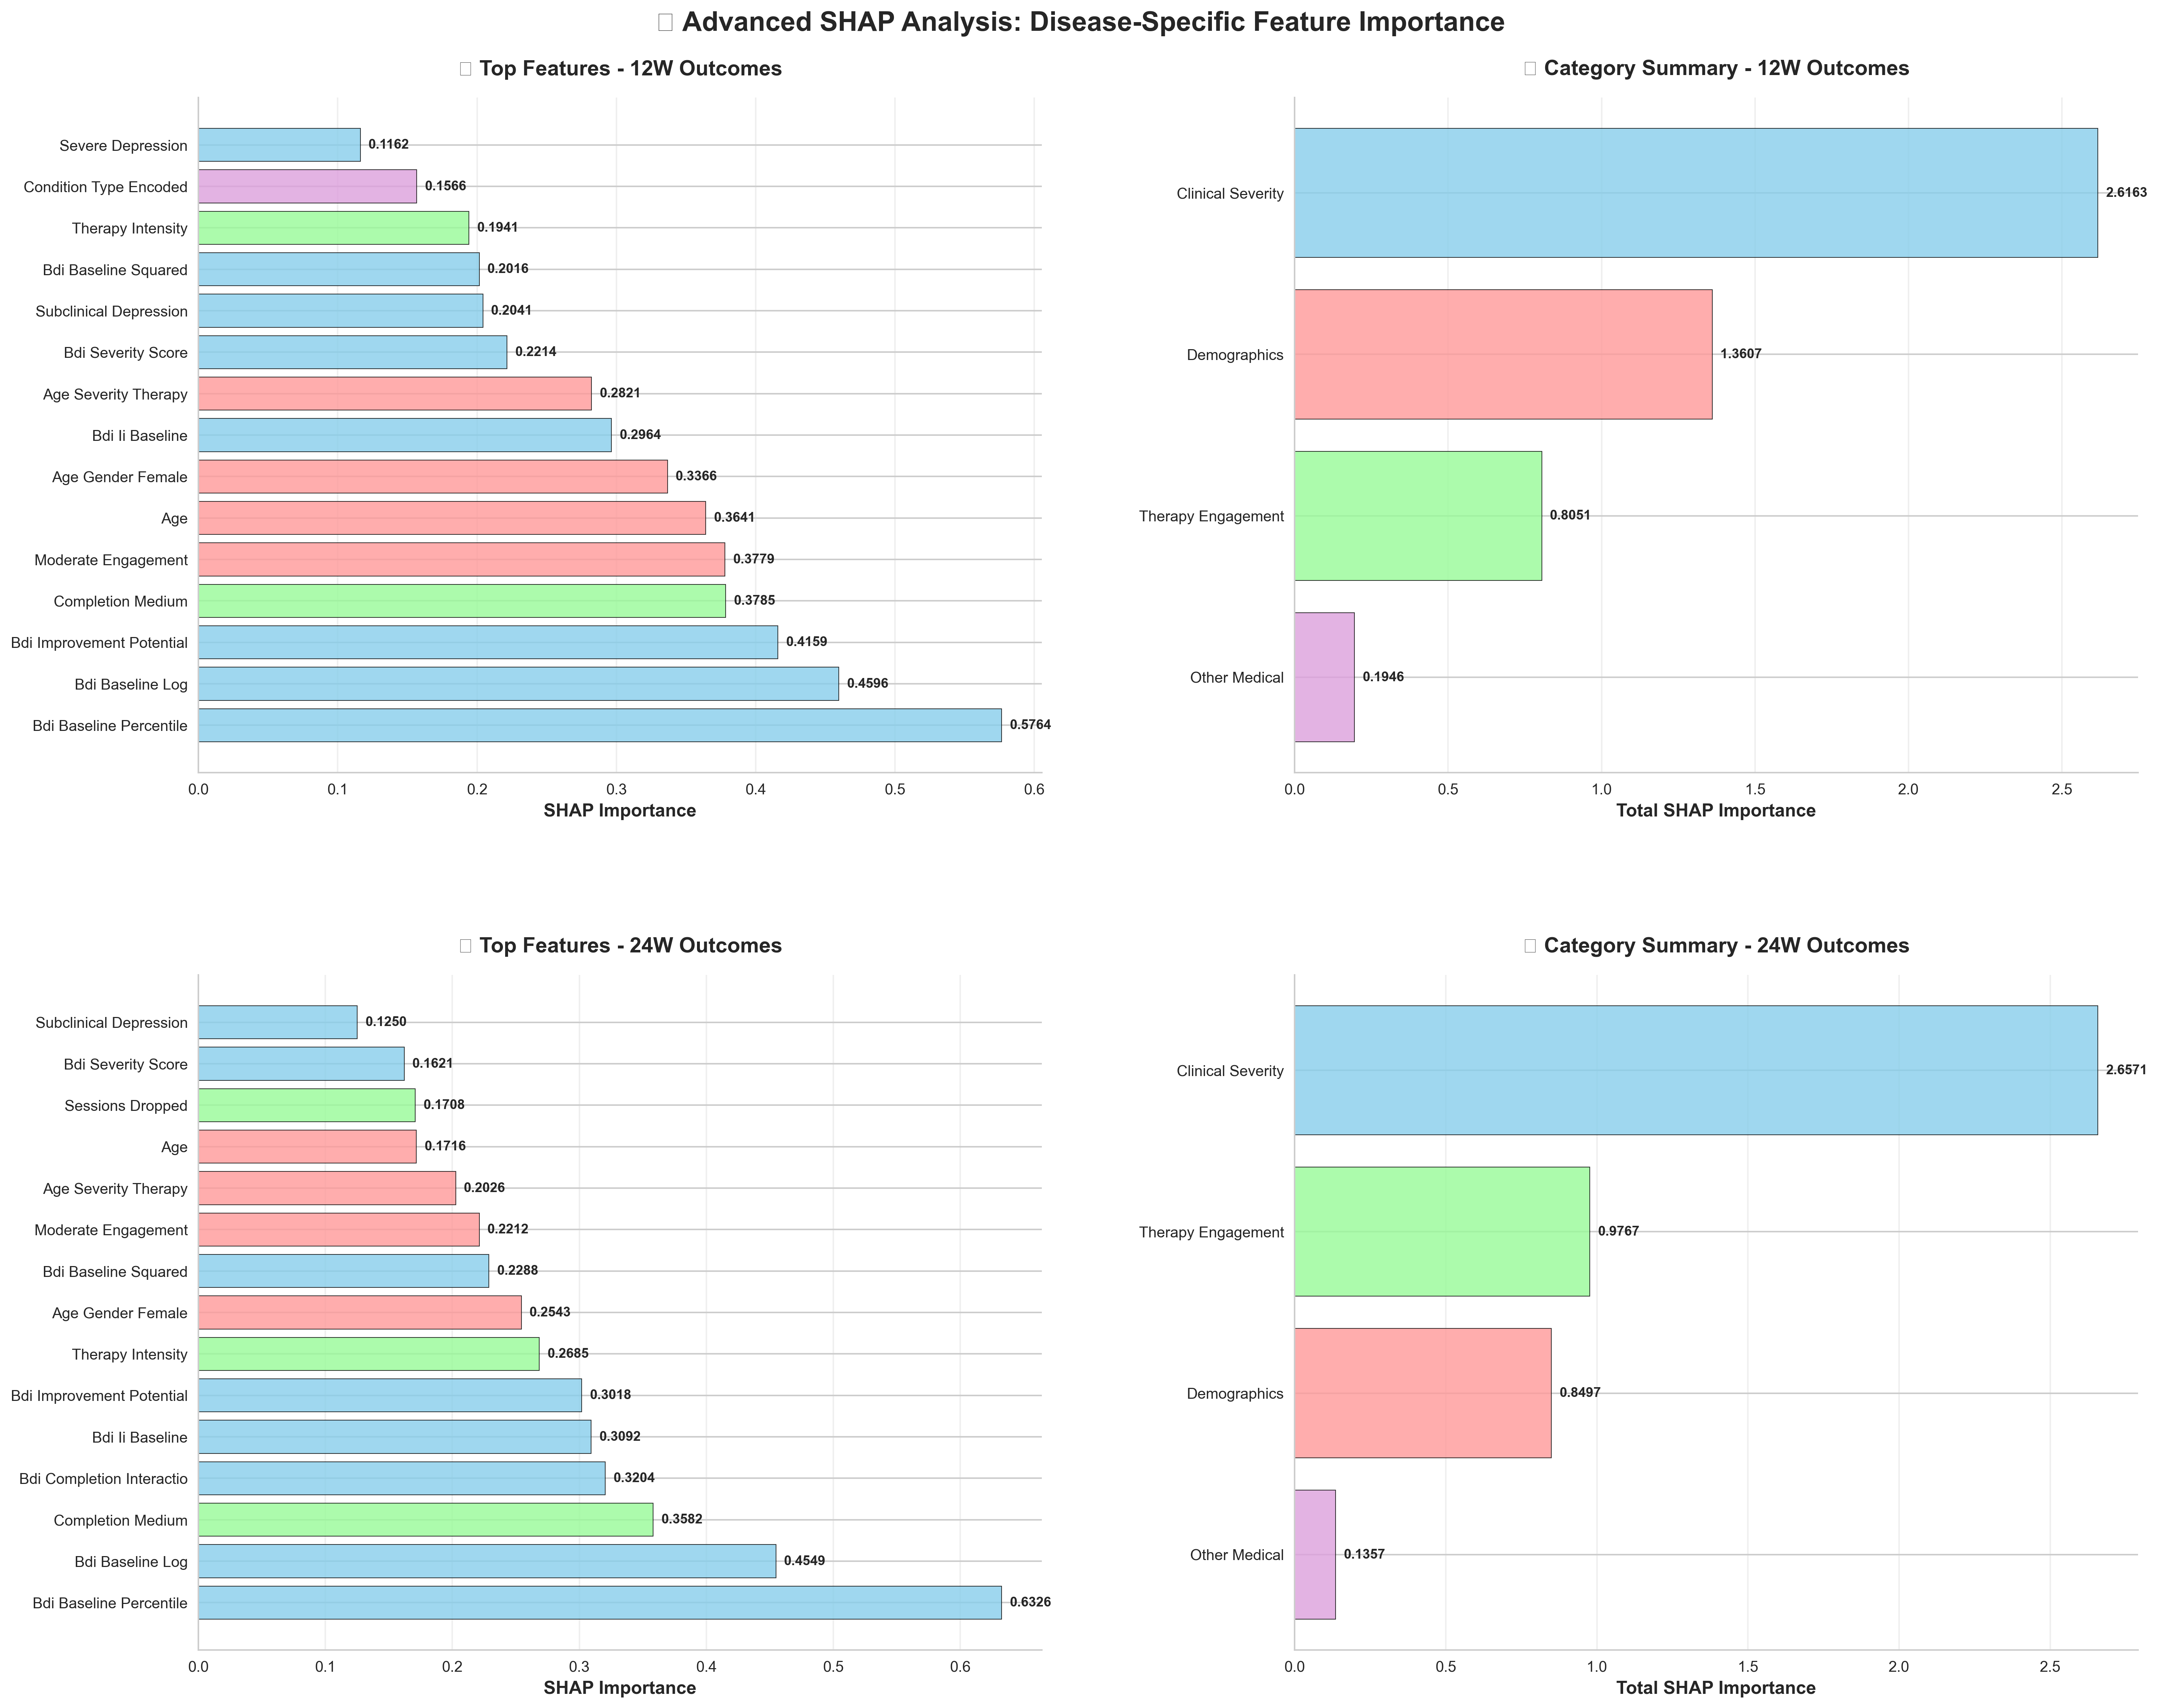
\includegraphics[width=0.48\textwidth]{figures/shap_feature_importance_static.png}
\caption{Global SHAP feature importance. Baseline BDI-II dominates.}
\label{fig:shap_global}
\end{figure}

\begin{figure}[h]
\centering
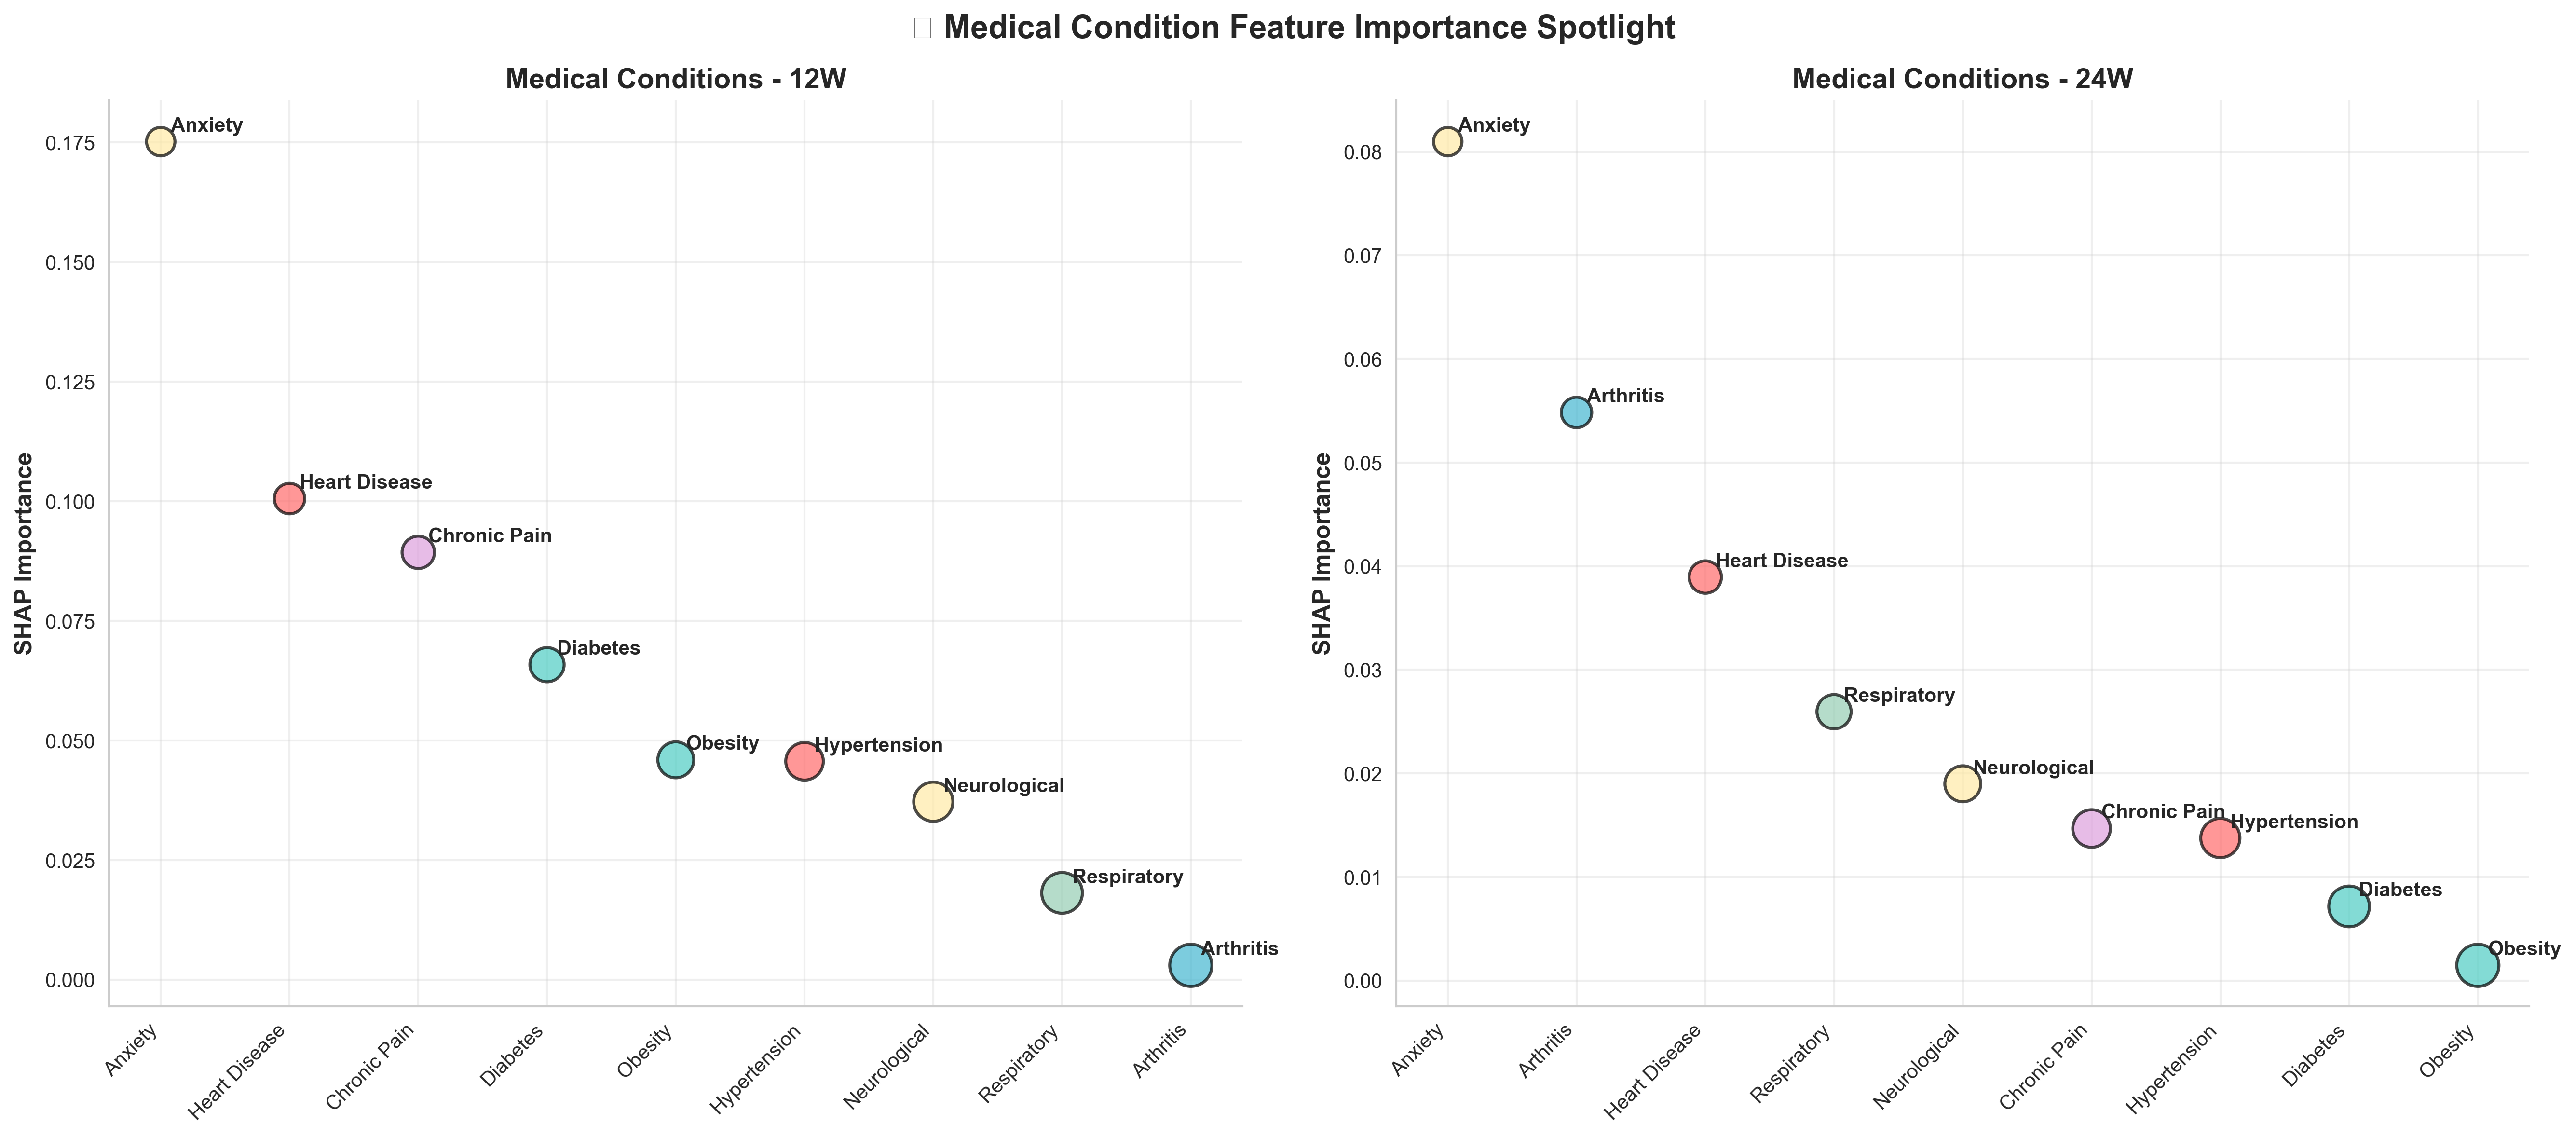
\includegraphics[width=0.48\textwidth]{figures/medical_conditions_shap_spotlight.png}
\caption{Medical condition SHAP impacts. Cancer increases risk, renal protective.}
\label{fig:shap_conditions}
\end{figure}

\section{Disease-Specific Analysis}

Medical comorbidities significantly moderate outcomes (Table~\ref{tab:descriptive}). \textbf{Cancer patients} (64.7\%, n=108) exhibit elevated depression: mean BDI = 8.51 vs. 5.59 (non-cancer), difference = +2.92, p = 0.007, Cohen's d = 0.41. This moderate effect persists at 24W (+3.31, p = 0.001), indicating sustained cancer-related psychological burden requiring augmented interventions.

\textbf{Renal insufficiency} (6.0\%, n=10) shows protective patterns: mean BDI = 3.50 vs. 7.73, difference = -4.23, p = 0.017, d = -0.59. Despite small sample size, the significant moderate effect persists at 24W (p = 0.046), potentially reflecting intensive monitoring, structured adherence, or resilience from chronic disease management.

\textbf{Lower limb amputation} (6.0\%, n=10) demonstrates neutral effects: mean BDI = 8.50 vs. 7.41 (non-amputation), difference = +1.09, p = 0.884, d = 0.15. The small non-significant effect indicates amputation status alone does not substantially predict depression outcomes. At 24W, a trend toward improvement emerges (difference = -1.93, p = 0.351), though remains non-significant, suggesting adaptation or prosthetic rehabilitation benefits may require longer observation.

\textbf{Acute coronary syndrome} (23.4\%, n=39) trends toward lower depression at 12W (5.38 vs. 8.12, p = 0.071), reaching significance by 24W (p = 0.044, d = -0.32), possibly from cardiac rehabilitation benefits (Table~\ref{tab:condition_analysis}).

Disease-stratified models achieve excellent within-group performance (12W): Cancer R² = 0.928 (MAE = 1.55), Cardiovascular R² = 0.812 (MAE = 1.65), Renal R² = 0.922 (MAE = 1.20), suggesting condition-specific prediction strategies enhance personalization.

\subsection{Therapy Engagement by Medical Condition}

Therapy engagement exhibits condition-specific patterns with differential impacts on outcomes (Table~\ref{tab:therapy_engagement}). Cancer patients demonstrate highest engagement (completion rate: 77.2\% vs. 49.9\% non-cancer, p<0.001, d=0.87) and derive significant benefit: 24W therapy-BDI correlation r=-0.232 (p=0.016), with high-engagement patients showing 4.19-point lower BDI scores (p=0.014). Conversely, ACS patients show lowest engagement (49.1\% completion) and paradoxical positive correlations at 24W (ρ=+0.374, p=0.019), likely reflecting reverse causation where symptomatic patients increase therapy participation. Renal patients exhibit similar paradoxical patterns (r=+0.656, p=0.039) despite excellent baseline outcomes (BDI=3.5), suggesting intensive medical monitoring provides primary protective effects. Amputation patients show low engagement (43.8\%) with no significant therapy-outcome associations, indicating physical rehabilitation priorities supersede mindfulness interventions. These findings support condition-stratified intervention protocols: maximize therapy access for cancer patients while investigating alternative approaches for cardiovascular and musculoskeletal conditions.

\begin{table}[h]
\centering
\caption{Therapy Engagement and Depression Outcomes by Medical Condition}
\label{tab:therapy_engagement}
\resizebox{\columnwidth}{!}{%
\begin{tabular}{@{}lccccccc@{}}
\toprule
\textbf{Condition} & \textbf{N} & \textbf{Comp.} & \textbf{Engage.} & \textbf{r\textsubscript{12W}} & \textbf{r\textsubscript{24W}} & \textbf{p\textsubscript{24W}} & \textbf{Effect} \\ 
 & & \textbf{Rate} & \textbf{vs Non} & \textbf{(BDI)} & \textbf{(BDI)} & & \textbf{(Hi-Lo)} \\
\midrule
Cancer & 108 & 77.2\% & +27.4\%*** & -0.133 & \textbf{-0.232*} & \textbf{0.016} & \textbf{-4.19*} \\
ACS & 39 & 49.1\% & -24.0*** & -0.114 & +0.374* & \textbf{0.019} & \textbf{+2.83*} \\
Renal & 10 & 58.7\% & -9.1\% & +0.466 & \textbf{+0.656*} & \textbf{0.039} & +3.40 \\
Amputation & 10 & 43.8\% & -25.3\% & +0.354 & +0.333 & 0.346 & +3.80 \\
\bottomrule
\end{tabular}%
}
\begin{tablenotes}
\footnotesize
\item Comp. Rate = therapy completion rate; Engage. vs Non = difference from patients without condition; r = Pearson correlation (Spearman for ACS 24W); Effect (Hi-Lo) = BDI difference between high vs low engagement groups at 24W; * p<0.05, ** p<0.01, *** p<0.001
\end{tablenotes}
\end{table}

\begin{table}[h]
\centering
\caption{Descriptive Statistics by Disease Group (12W BDI)}
\label{tab:descriptive}
\resizebox{\columnwidth}{!}{%
\begin{tabular}{@{}lccccc@{}}
\toprule
\textbf{Disease} & \textbf{N} & \textbf{Mean} & \textbf{SD} & \textbf{Median} & \textbf{Q1-Q3} \\ \midrule
Cancer & 108 & 8.51 & 7.68 & 7.0 & 3.0–12.3 \\
Cardiovascular & 39 & 5.38 & 5.11 & 3.0 & 1.0–8.0 \\
Renal & 10 & 3.50 & 6.13 & 1.0 & 0.0–4.0 \\
Musculoskeletal & 10 & 8.50 & 8.67 & 7.0 & 0.8–12.5 \\ \bottomrule
\end{tabular}%
}
\end{table}

\begin{table}[h]
\centering
\caption{Individual Condition Statistical Analysis (12W)}
\label{tab:condition_analysis}
\resizebox{\columnwidth}{!}{%
\begin{tabular}{@{}lccccc@{}}
\toprule
\textbf{Condition} & \textbf{N} & \textbf{With} & \textbf{Without} & \textbf{Diff} & \textbf{p} \\ \midrule
Cancer & 108 & 8.51 ± 7.68 & 5.59 ± 6.07 & +2.92 & \textbf{0.007} \\
Renal & 10 & 3.50 ± 6.13 & 7.73 ± 7.28 & -4.23 & \textbf{0.017} \\
Amputation & 10 & 8.50 ± 8.67 & 7.41 ± 7.20 & +1.09 & 0.884 \\
ACS & 39 & 5.38 ± 5.11 & 8.12 ± 7.72 & -2.73 & 0.071 \\ \bottomrule
\end{tabular}%
}
\end{table}

\section{Early Insights and Future Directions}

\textbf{Key Findings:} (1) Timepoint-specific architectures optimize performance—Transformer for 12W temporal patterns, CatBoost for 24W long-term robustness. (2) Medical comorbidity critically moderates outcomes: cancer increases depression (+2.92, p=0.007), renal shows protection (-4.23, p=0.017). (3) Therapy engagement exhibits condition-specific effects: cancer patients benefit significantly (r=-0.232, p=0.016; high-engagement reduces BDI by 4.19 points), while cardiovascular patients show paradoxical patterns requiring alternative interventions. (4) Modest R² (0.20-0.25) represents meaningful progress for multifactorial depression prediction. (5) Baseline BDI-II dominates (35-45\%), yet remaining variance highlights actionable intervention targets.

\textbf{Ongoing Work:} Meta-ensemble combining Transformer+CatBoost; trajectory phenotyping for outcome subtypes; uncertainty quantification via conformal prediction; external validation on independent cohorts.

\textbf{Submission Strategy:} Dual-model system with disease-stratified predictions, condition-specific therapy recommendations, SHAP explanations, and uncertainty estimates for high-risk flagging.

\section{Conclusion}

This preliminary analysis establishes a systematic multi-phase framework evaluating 38 models for depression outcome prediction. Timepoint-specific architectures achieve optimal performance: Transformer for 12W (R² = 0.247) and CatBoost for 24W (R² = 0.200). Disease-specific analysis reveals significant condition-dependent effects (cancer: +2.92, p=0.007; renal: -4.23, p=0.017) with therapy engagement showing condition-stratified impacts: cancer patients derive substantial benefit (r=-0.232, p=0.016), while cardiovascular conditions exhibit paradoxical patterns warranting alternative approaches. SHAP interpretability identifies baseline severity, age, and treatment engagement as key predictors. These findings provide a foundation for clinically deployable prediction systems supporting personalized treatment planning and risk stratification. Ongoing work focuses on ensemble integration, trajectory phenotyping, and external validation.

\section*{Acknowledgment}
We thank the IEEE EMBS BHI 2025 organizers for providing this valuable dataset and competition framework.

\begin{thebibliography}{00}
\bibitem{beck1996manual} A. T. Beck, R. A. Steer, and G. K. Brown, \textit{Manual for the Beck Depression Inventory-II}. San Antonio, TX: Psychological Corporation, 1996.

\bibitem{pizzagalli2005reduced} D. A. Pizzagalli et al., ``Reduced caudate and nucleus accumbens response to rewards in unmedicated individuals with major depressive disorder,'' \textit{American Journal of Psychiatry}, vol. 162, no. 6, pp. 1198–1205, 2005.

\bibitem{treadway2009worth} M. T. Treadway and D. H. Zald, ``Reconsidering anhedonia in depression: Lessons from translational neuroscience,'' \textit{Neuroscience \& Biobehavioral Reviews}, vol. 35, no. 3, pp. 537–555, 2011.

\bibitem{wang2013psychometric} Y. P. Wang and C. Gorenstein, ``Psychometric properties of the Beck Depression Inventory-II: A comprehensive review,'' \textit{Brazilian Journal of Psychiatry}, vol. 35, no. 4, pp. 416–431, 2013.

\bibitem{hunot2013mindfulness} V. Hunot et al., ``Mindfulness-based `third wave' cognitive and behavioural therapies versus other psychological therapies for depression,'' \textit{Cochrane Database of Systematic Reviews}, 2013.

\end{thebibliography}

\end{document}
